\documentclass{beamer}
\usepackage{graphicx}
\usepackage{bm}
\usetheme{Boadilla}
\title{Preliminary concepts for taxonomic aggregation using modified isometric log ratio transformation (ILR)}
\author{Quang Nguyen}
\institute{Dartmouth College}

\begin{document}
\begin{frame}
    \titlepage 
\end{frame}

\begin{frame}
    \frametitle{Microbiome data is strictly compositional}
    \begin{itemize}
        \item All short read sequencing data exists as relative abundances
        \item RNASeq-type data sets usually can rely on certain assumptions about the relative consistent expression of housekeeping genes (e.g. DESeq2) or specific measurements of the PCR process (UMI counts in scRNAseq)
        \item Analysis of microbiome data hence relies on log-ratio based analyses from the compositional data analysis literature.  
    \end{itemize}
\end{frame}

\begin{frame}
    \frametitle{Microbiome analysis involves a lot of aggregation}
    \begin{columns}
        \begin{column}{0.5\textwidth}
            \begin{itemize}
                \item Most often, variables are aggregated to the Linnean taxonomic tables 
                \item \textbf{Note:} Phylogeny and taxonomy generally agrees, however this is not always the case. 
                \item Aggregating variables to pre-defined sets describes a class of methods known as gene set analysis (GSA).  
            \end{itemize}
        \end{column}
        \begin{column}{0.5\textwidth}
            \begin{center}
                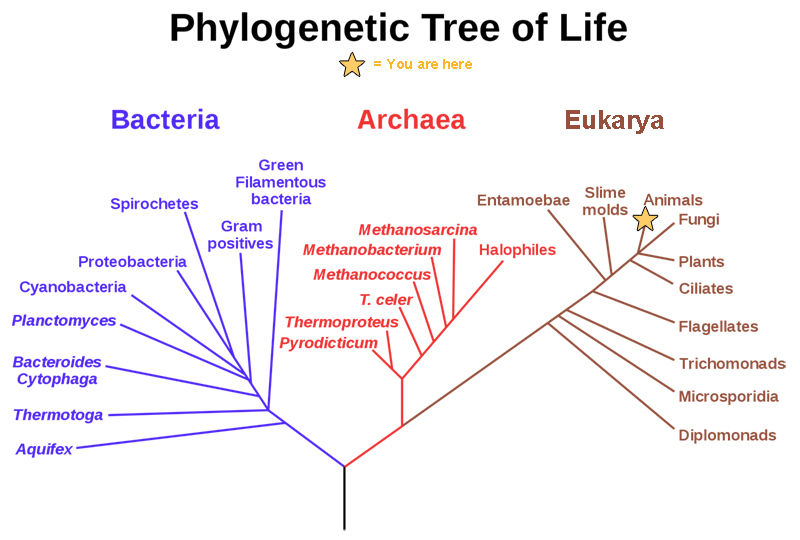
\includegraphics[scale=0.25]{taxonomic_tree.png}
            \end{center}
        \end{column}
    \end{columns}
\end{frame}



\begin{frame}
    \frametitle{Typical analysis involves summation of relative abundances (or raw counts)}
    \begin{itemize}
        \item This approach might cause problems 
        \begin{itemize}
            \item The compositional center is changed. For example, take a simple composition of 3 parts $x = [x_1, x_2, x_3]$ and the aggregated composition $y = [x_1 + x_2, x_3]$ (with $n$ samples). The center \cite{aitchison} of the initial composition is 
            \[cen(x) = \mathcal{C}\left[ (\prod^n x_1)^{1/n}, (\prod^n x_2)^{1/n}, (\prod^n x_3)^{1/n} \right]\]
            while the center of the aggregated composition is 
            \[cen(y) = \mathcal{C}\left[ (\prod^n (x_1 + x_2))^{1/n}, (\prod^n x_3)^{1/n} \right]\]
            \item This results in the lack of preservation for inter-sample distances following aggregation, and the relationship is non-monotonic \cite{egozcue2005}.  
        \end{itemize}
    \end{itemize}
\end{frame}

\begin{frame}
    \frametitle{Isometric log-ratio transformation}
    \begin{columns}
        \begin{column}{0.5\textwidth}
            \begin{itemize}
                \item Defined as a transformation of of the composition in the simplex $S^D$ to $\mathcal{R}^{D-1}$ by projecting onto an Aichison orthonormal basis. 
                \item Prior researchers have proved \cite{egozcue2003} that such a basis can be constructed from a sequential binary partition (SBP) or a tree - each variable is therefore defined as a "balance" \cite{morton2017a}
            \end{itemize}
        \end{column}
        \begin{column}{0.5\textwidth}
            \begin{center}
                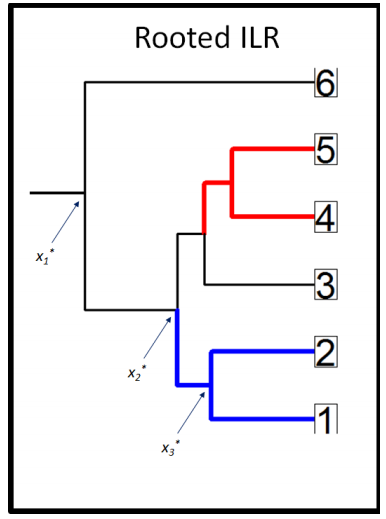
\includegraphics[scale=0.5]{phylogeny_demonstration.png}
            \end{center}
        \end{column}
    \end{columns}
\end{frame}

\begin{frame}
    \frametitle{Isometric log-ratio transformation}
    \begin{columns}
        \begin{column}{0.6\textwidth}
            \begin{itemize}
                \item ILR statistic is defined as 
                \begin{equation}
                    x^*_{R/S} = \sqrt{\frac{rs}{r+s}} \log(\frac{g(\bm{y}_R)}{g(\bm{y}_S)}
                \end{equation}
                \item $g(\bm{y}_R)$ indicates the geometric mean of all $y_i$ for $i \in R$ 
                \item The basis defined by the $R/S$ partition is \[\bm{e}_i = \mathcal{C}[\exp(0,..,\underbrace{a,..., a}_{r \text{ elements}},\overbrace{b,...,b}^{s \text{ elements}},...,0))] \]  
                where $a = \sqrt{\frac{r}{(r + s) \cdot s}}$ and $b = \sqrt{\frac{-s}{(r+s) \cdot r}}$
            \end{itemize}
        \end{column}
        \begin{column}{0.4\textwidth}
            \begin{center}
                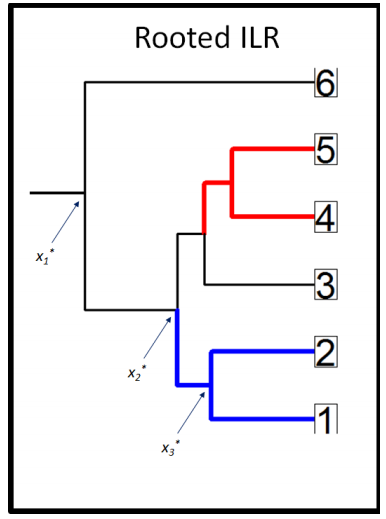
\includegraphics[scale=0.3]{phylogeny_demonstration.png}
            \end{center}
        \end{column}
    \end{columns}
\end{frame}

\begin{frame}
    \frametitle{Competitive gene set testing using isometric log ratio transformation}
    \begin{itemize}
        \item $\bm X$: The $n \times p$ matrix of relative abundances of $p$ LT proportions in $n$ samples
        \item $\bm A$: The $m \times p$ matrix denoting the assignment of $p$ LT proportions into $m$ HT sets
    \end{itemize}
    We generate the following matrix: 
    \begin{itemize}
        \item $\bm S$: The $n \times m$ matrix denoting the enrichment scores of $m$ HT sets by $n$ samples. 
    \end{itemize}
\end{frame}


\begin{frame}
    With inputs $\bm{X}$ and $\bm{A}$, we compute $\bm{S}$ as follows:  
    \frametitle{Competitive gene set testing using isometric log ratio transformation}
    \begin{enumerate}
        \item Let $\bm{R}$ be a $n \times m$ matrix of competitive $ilr$ statistic for each HT set which is defined as follows:
        \begin{equation}
        R_{ij} = \sqrt{\frac{\sum_k A_{jk}(p - \sum_k A_{jk})}{p}} \log \left(\frac{g(\bm{x}_{ik} |A_{jk} \neq 0)}{g(\bm{x}_{ik} | A_{jk} = 0)}\right)
        \end{equation}
        \item To capture the distribution of the $ilr$ test statistic under the null hypothesis that the relative weights of LT proportions in the HT sets to the overall composition is no different than LT proportions not in the HT sets, the competitive $ilr$ statistic is computed for each HT set with permuting row labels of matrix $\bm{A}$, simulating random assignments of LTs into HT sets. Denote $\bm{A}_{perm}$ be the row-permuted version of $\bm{A}$ and $\bm{R}_{perm}$ be row-permuted version of $\bm{R}$
    \end{enumerate}
\end{frame}

\begin{frame}
    \frametitle{Competitive gene set testing using isometric log ratio transformation}
    \begin{enumerate}
        \item We fit a gaussian distribution using the method of maximum likelihood for each column $\bm{R}_{perm}$. This stem from previous research treating the $ilr$ coordinates as normally distributed \cite{egozcue2005}.  
        \item Calculate a $z$-score using the fitted null distribution to compute HT specific enrichment scores. We formulate the target matrix $S$ as $z$-scores for the normal distribution fitted on columns of $\bm{R}_{perm}$:
        \begin{equation}
            \bm{S}[,k] = (\bm{R}[,k] - \hat{\mu}_{\mathcal{N}_{\bm{R}_{perm}}})/\hat{\sigma}_{\mathcal{N}_{\bm{R}_{perm}}}
        \end{equation}
    \end{enumerate}
\end{frame}

\begin{frame}
    \frametitle{Statistical interpretation of this statistic}
    \begin{itemize}
        \item Projecting the original composition onto the axis defined by the balance between taxa within the higher taxonomic set and those who are not. 
        \item Equivalent to defining an $ilr$ transform on a set of SBPs such that the first order split is between members of the set and the remaining variables. 
        \item These coordinates are on the same scale, and is no longer bound by the composition. The variable aggregation process is also compositionally coherent.   
    \end{itemize}
\end{frame}

\begin{frame}
    \frametitle{Early Results}
    \begin{columns}
        \begin{column}{0.5\textwidth}
            \begin{itemize}
                \item Density estimation for the null with 100 column permutations
                \item Mean: -0.07, SD: 1.5
            \end{itemize}
        \end{column}
        \begin{column}{0.5\textwidth}
            \begin{center}
                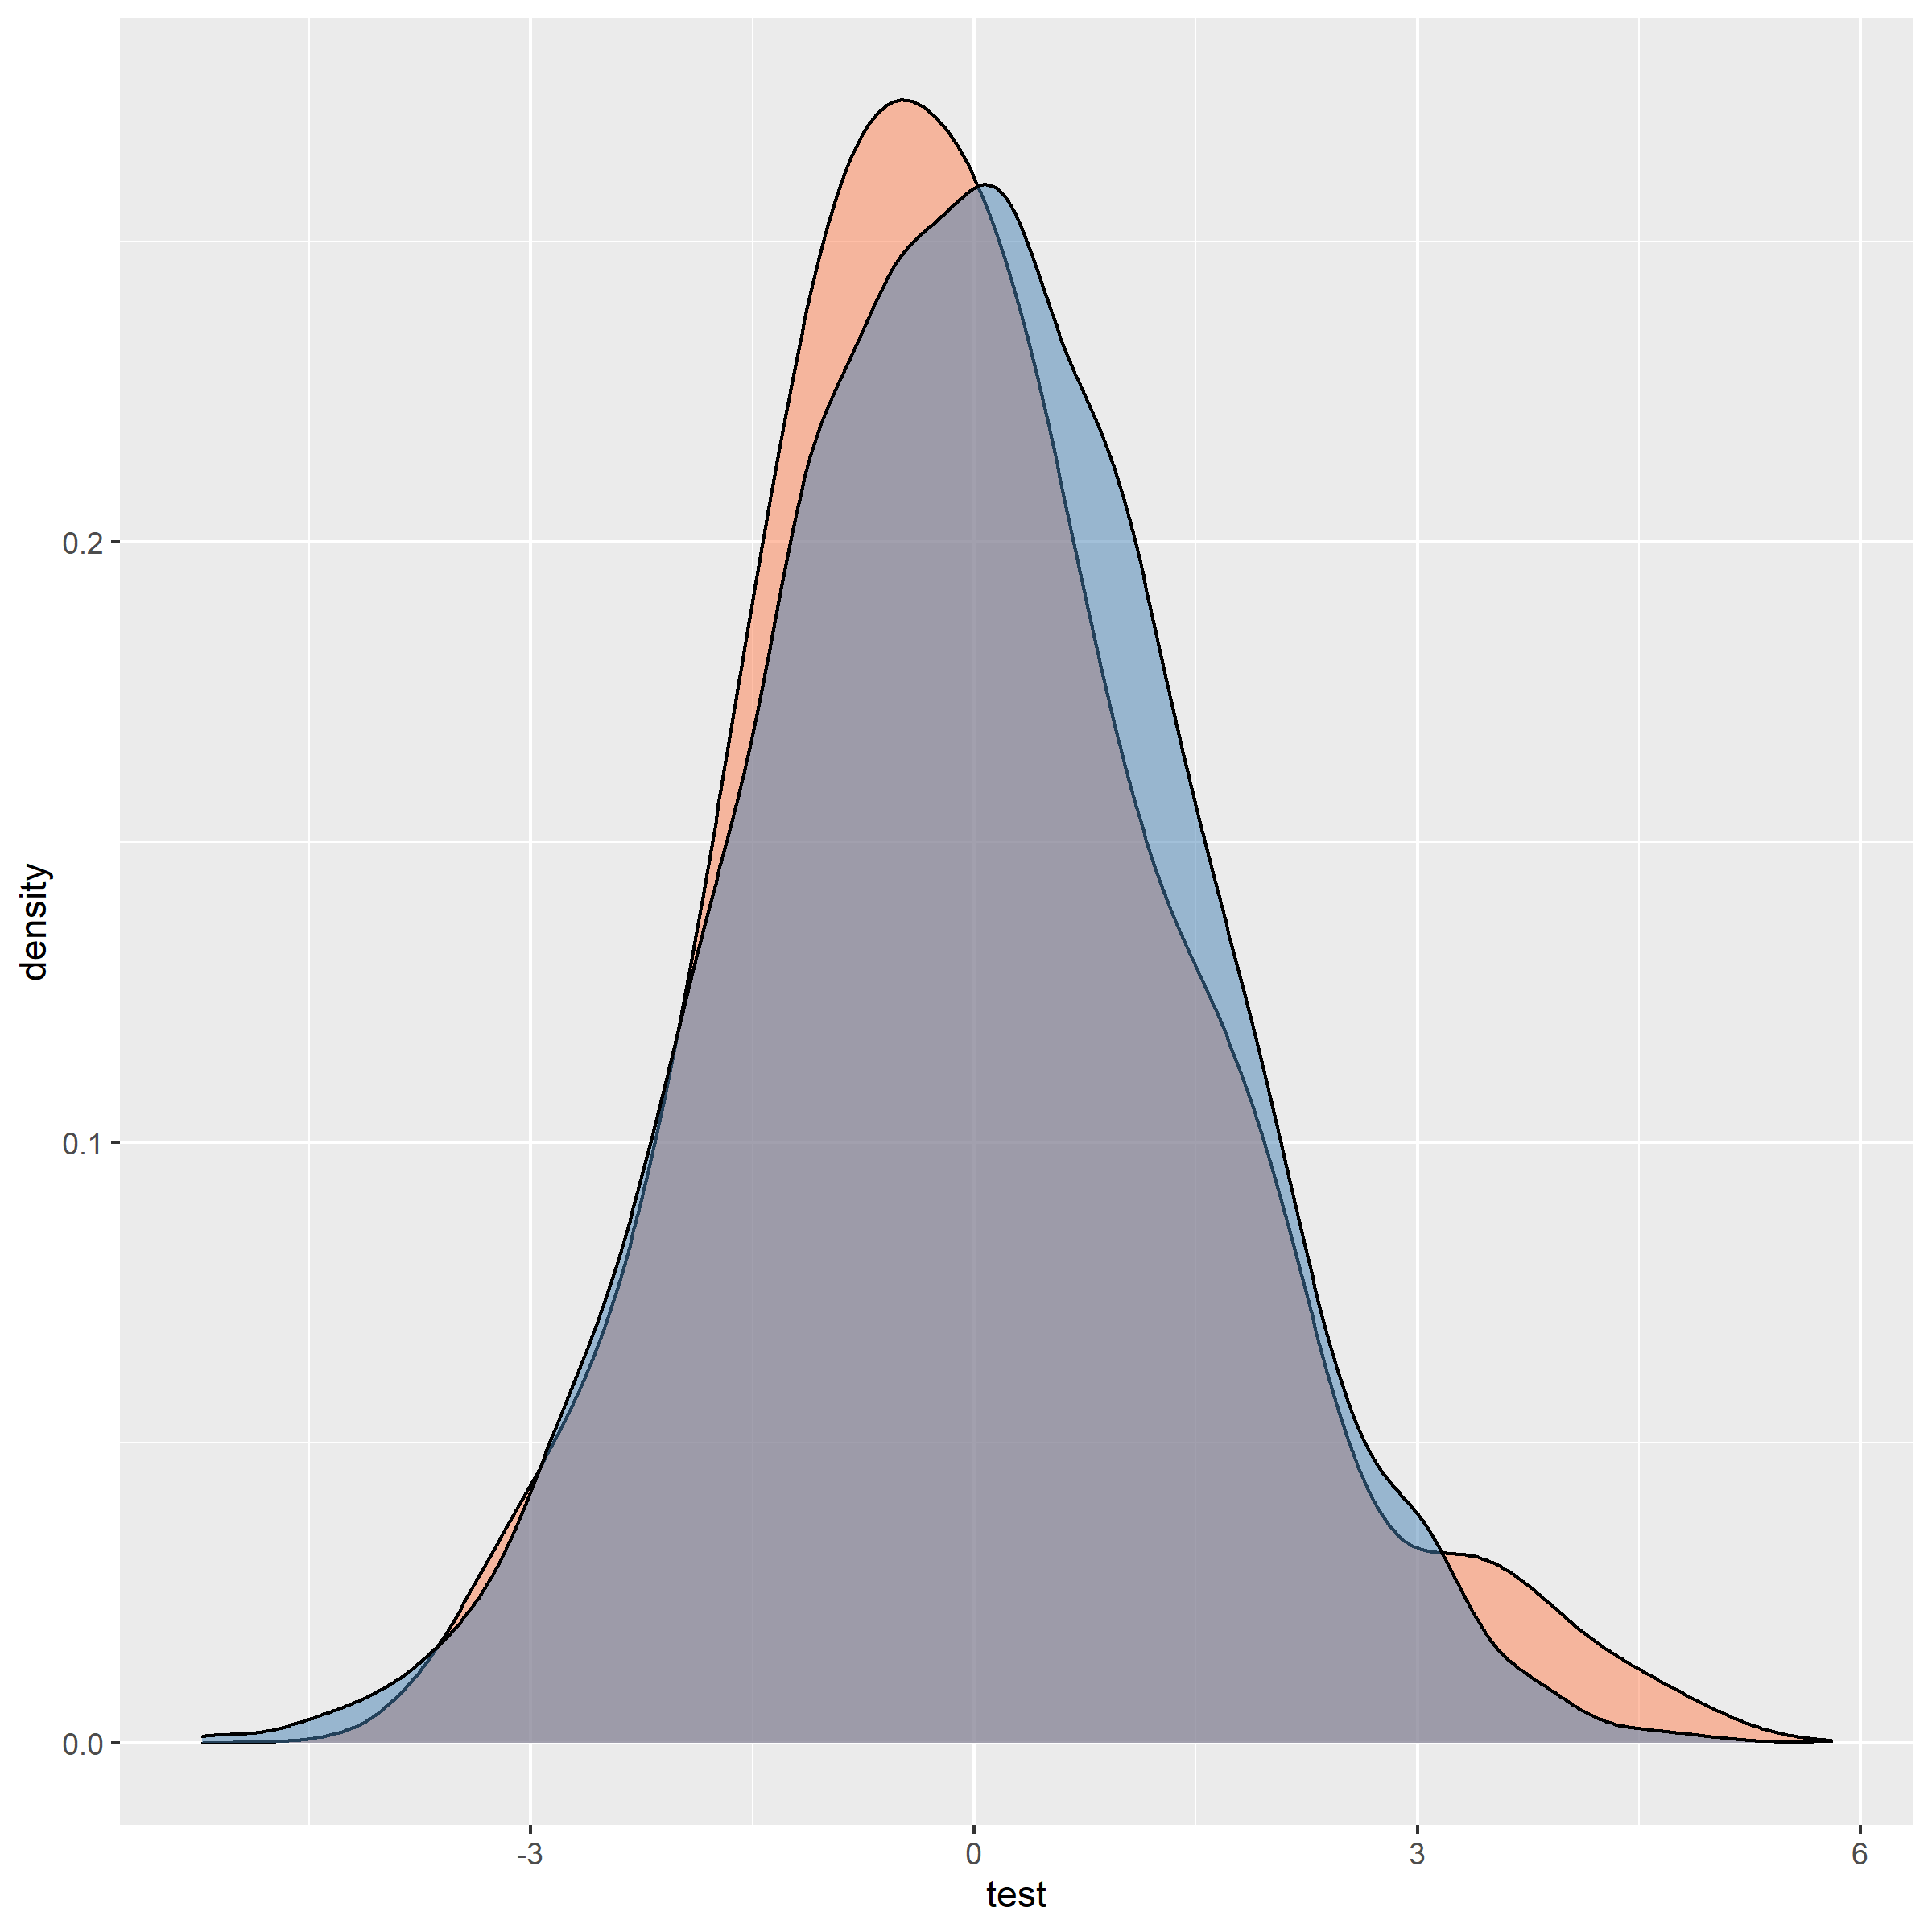
\includegraphics[scale=0.325]{figures/null_density.png}
            \end{center}
        \end{column}
    \end{columns}
\end{frame}


\begin{frame}
    \frametitle{Early Results}
    \begin{columns}
        \begin{column}{0.5\textwidth}
            \begin{itemize}
                \item GlobalPatterns data set. 
                \item Genus level aggregation 
                \item Euclidean distances (after $clr$ transformation for simple summation counts)
            \end{itemize}
        \end{column}
        \begin{column}{0.5\textwidth}
            \begin{center}
                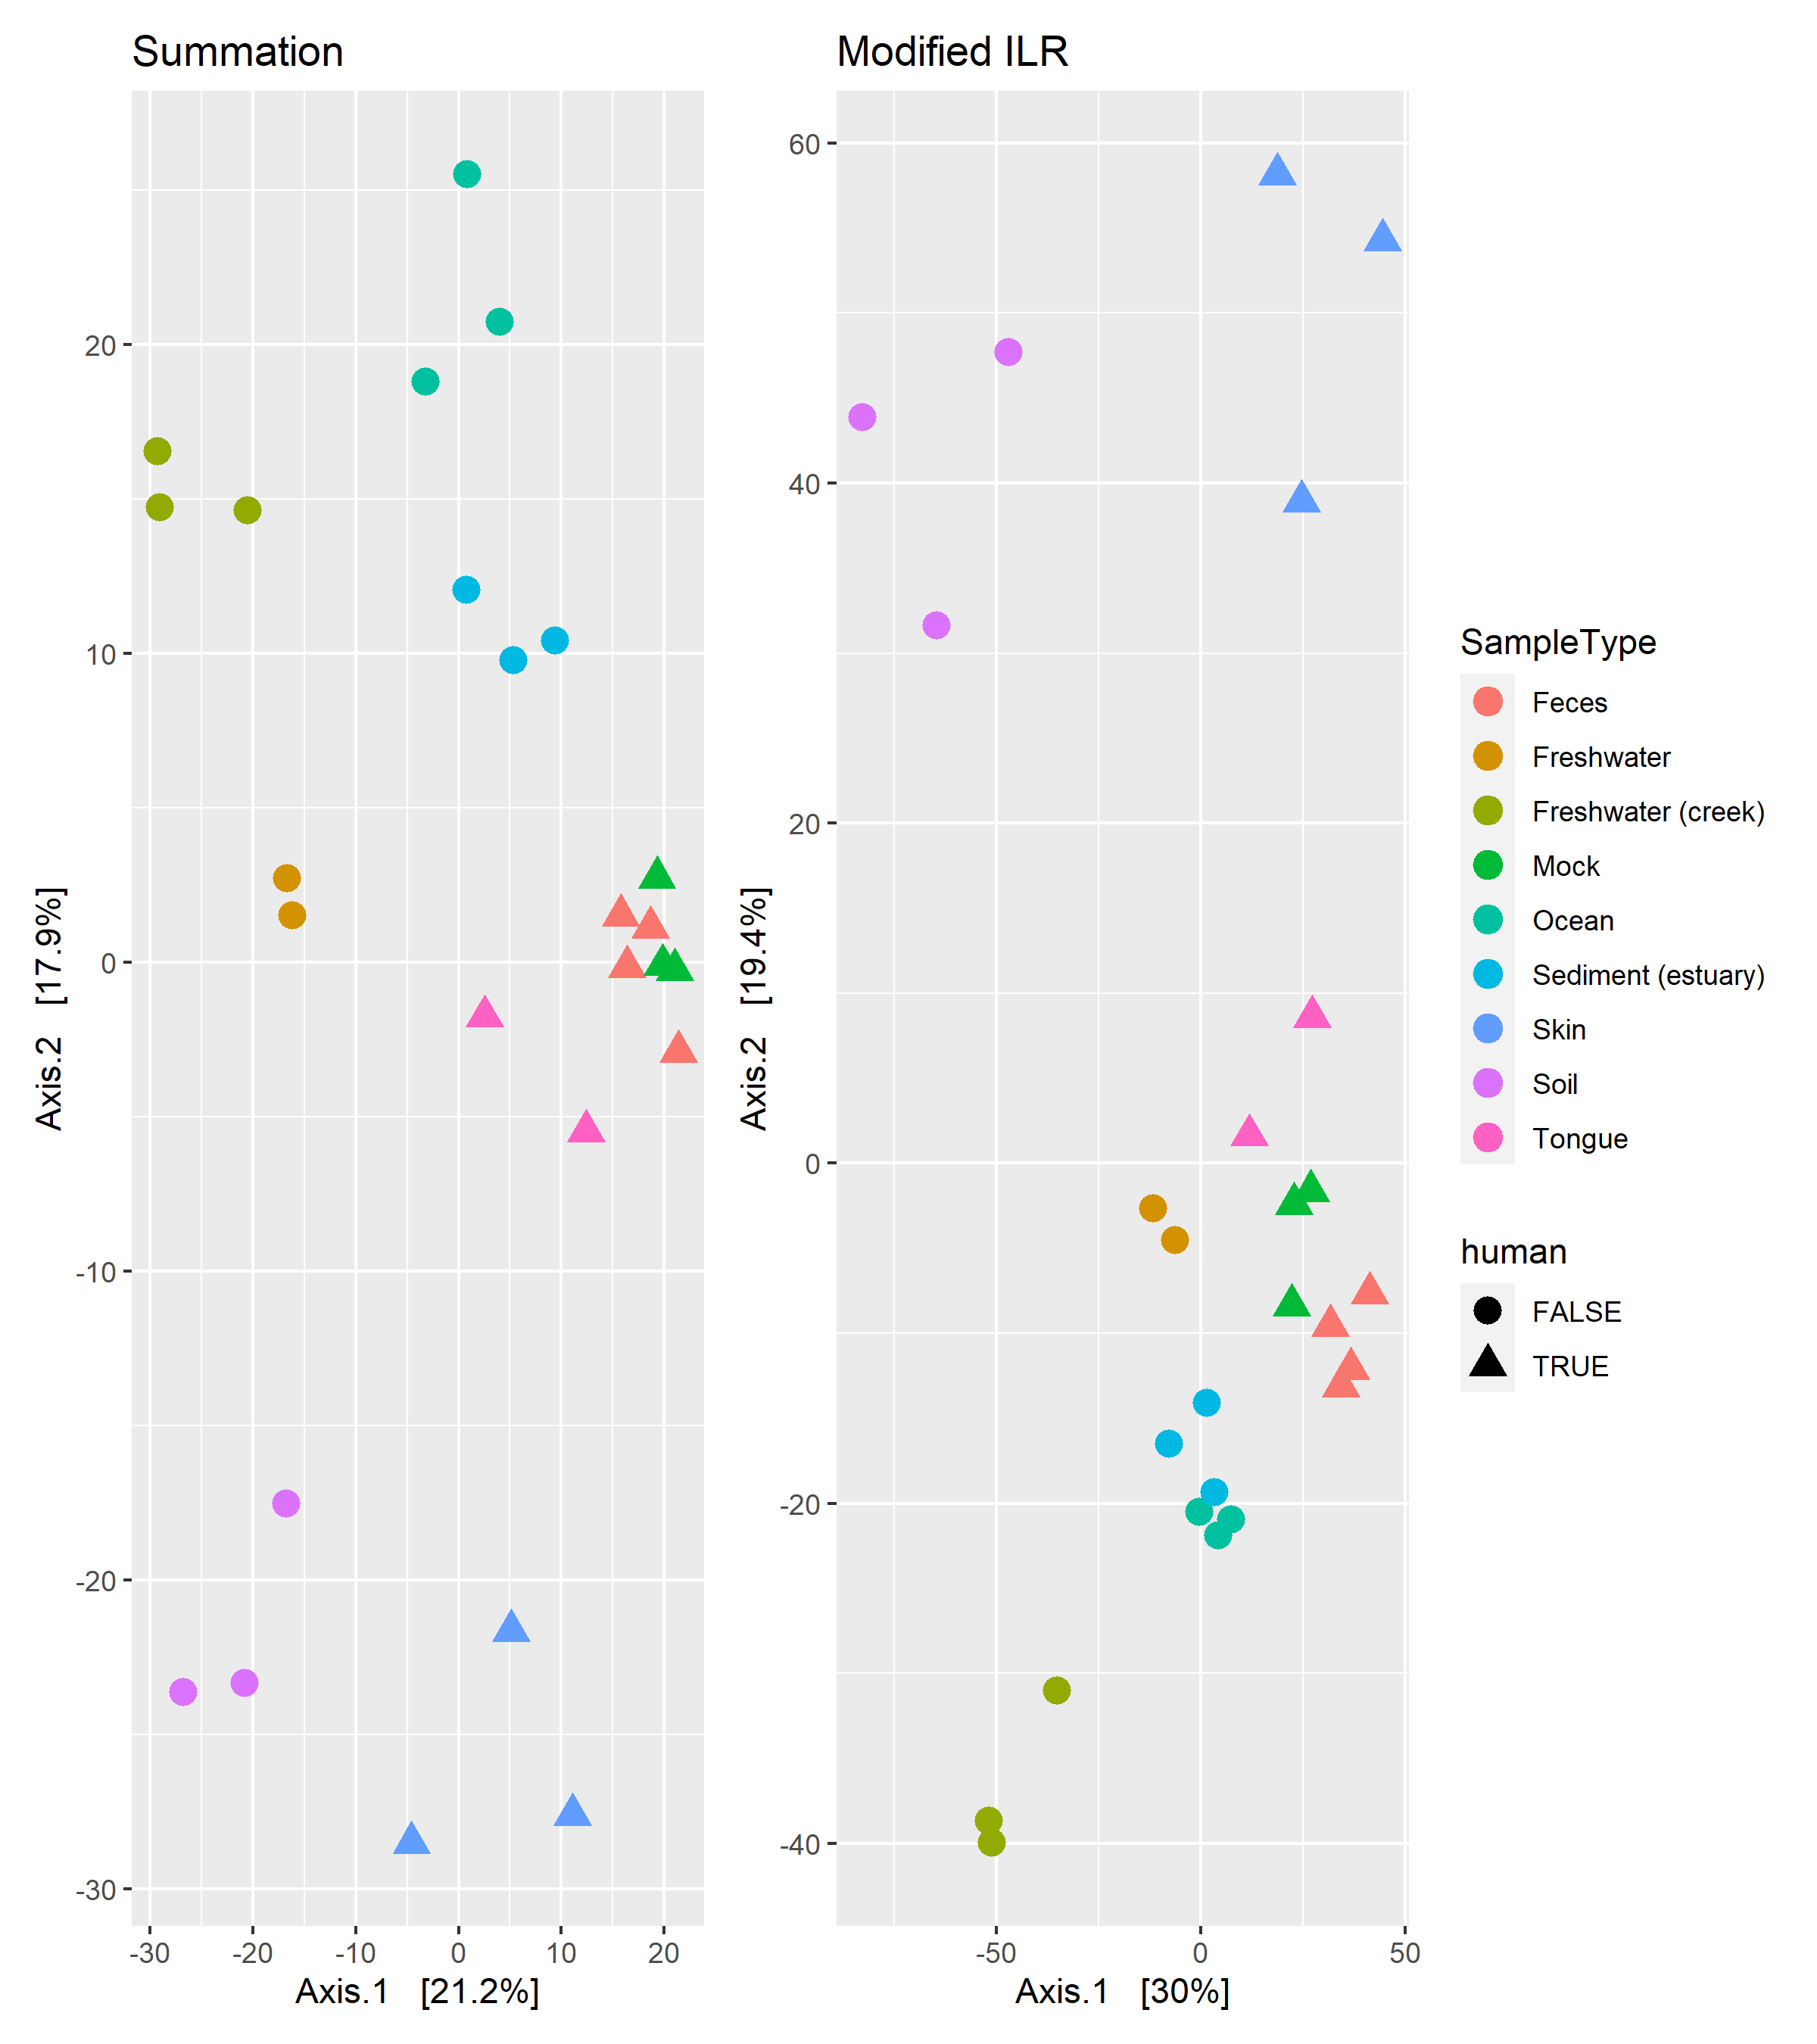
\includegraphics[scale=0.325]{figures/prelim_results.png}
            \end{center}
        \end{column}
    \end{columns}
\end{frame}

\begin{frame}
    \frametitle{Disadvantages}  
    \begin{itemize}
        \item Does not deal with true hierarchical structure
        \item Did not take into account phylogeny 
        \item Unsure about justification above using simple sum 
        \item Some uncertainties about correlation
    \end{itemize}
\end{frame}


\begin{frame}
    \frametitle{Next Steps}  
    \begin{itemize}
        \item Implement the resampling procedure in the prototype
        \item Dealing with singletons and inter-taxa correlation 
        \item Performing simulations to determine type I error and power. 
        \item Real data implementation  
    \end{itemize}
\end{frame}


\begin{frame}
    \frametitle{Bibliography}
    \bibliography{tax_agg}{}
    \bibliographystyle{plain}
\end{frame}


\end{document}